\documentclass[10pt,a4paper]{article}
\usepackage[a4paper,left=1.9cm,right=1.9cm,top=1.7cm,bottom=1.9cm,headsep=0.35cm,headheight=18pt]{geometry}
% Shared layout for report and factsheet (pdflatex, standard TeX Live / Overleaf packages)
\usepackage[T1]{fontenc}
\usepackage[utf8]{inputenc}
\usepackage[sc]{mathpazo}
\usepackage[scaled=0.9]{helvet}
\usepackage{microtype}
\usepackage{amsmath}
\usepackage{booktabs}
\usepackage{array}
\usepackage{tabularx}
\usepackage{graphicx}
\usepackage{xcolor}
\usepackage{enumitem}
\usepackage{caption}
\usepackage{titlesec}
\usepackage{fancyhdr}
\usepackage[hidelinks]{hyperref}

\definecolor{accent}{HTML}{1C5CAB}
\definecolor{muted}{HTML}{52514E}
\definecolor{rulegrey}{HTML}{C9C8C3}
\definecolor{panel}{HTML}{F3F2EE}

\newcommand{\TeamName}{Team Backwardation}
\newcommand{\TeamMembers}{Lukas Lobnig, Niklas Omann, Noemi Pirrello, Adrian Rupp}
\newcommand{\ProjectTitle}{Earning the Roll}
\newcommand{\ProjectSubtitle}{A volatility-targeted carry strategy for WTI crude oil futures}

% generated by wti.report - do not edit
\newcommand{\NNDaily}{9{,}145}
\newcommand{\NNWeekly}{1{,}909}
\newcommand{\NNRolls}{472}
\newcommand{\NRollAgree}{87\%}
\newcommand{\NRollAgreeN}{218}
\newcommand{\NRollBefore}{9\%}
\newcommand{\NRollAfter}{19\%}
\newcommand{\NKurtDaily}{16.5}
\newcommand{\NKurtMonthly}{2.4}
\newcommand{\NKurtResid}{2.2}
\newcommand{\NAcfAbsHundred}{0.06}
\newcommand{\NGarchSpec}{EGARCH-t}
\newcommand{\NGarchPersist}{0.991}
\newcommand{\NGarchNu}{6.8}
\newcommand{\NGarchGammaT}{\textminus 3.9}
\newcommand{\NGarchBicGain}{39}
\newcommand{\NDmEwmaP}{$<$0.001}
\newcommand{\NDmRollP}{$<$0.001}
\newcommand{\NDmNormalP}{0.316}
\newcommand{\NOvxCorr}{0.92}
\newcommand{\NVarLags}{4}
\newcommand{\NBicLags}{1}
\newcommand{\NAicLags}{8}
\newcommand{\NLbSlopeOne}{$<$0.001}
\newcommand{\NLbMinFour}{0.12}
\newcommand{\NGrangerAllP}{0.374}
\newcommand{\NGrangerSlopeP}{0.635}
\newcommand{\NPassSum}{0.0078}
\newcommand{\NPassZeroP}{0.482}
\newcommand{\NPassFullP}{0.305}
\newcommand{\NBackAnn}{26.7}
\newcommand{\NBackT}{3.1}
\newcommand{\NContAnn}{\textminus 14.1}
\newcommand{\NContT}{\textminus 1.2}
\newcommand{\NIrfSlopeInvImpact}{\textminus 0.72}
\newcommand{\NIrfSlopeInvTwelve}{\textminus 0.46}
\newcommand{\NIrfRetInvImpact}{\textminus 0.40}
\newcommand{\NIrfRetInvTwelve}{\textminus 0.29}
\newcommand{\NIrfRetSlopeImpact}{2.85}
\newcommand{\NIrfRetSlopeTwelve}{3.53}
\newcommand{\NIrfDrift}{0.68}
\newcommand{\NIrfDriftLo}{\textminus 0.25}
\newcommand{\NIrfDriftHi}{1.35}
\newcommand{\NSlopeSd}{6.1}
\newcommand{\NWeeklyVolIs}{4.6}
\newcommand{\NCarryWeekIs}{0.28}
\newcommand{\NBenchVolIs}{36.5\%}
\newcommand{\NOosRtwoVal}{\textminus 2.0\%}
\newcommand{\NOosRtwoOos}{\textminus 2.6\%}
\newcommand{\NCwPOos}{0.819}
\newcommand{\NVarShareLong}{58\%}
\newcommand{\NNTrials}{26}
\newcommand{\NDsrHurdle}{0.60}
\newcommand{\NDsr}{63\%}
\newcommand{\NTargetVol}{35\%}
\newcommand{\NMaxLev}{2}
\newcommand{\NFreezeCommit}{9fb1e8d}
\newcommand{\NHolmMain}{0.282}
\newcommand{\NPsrMainP}{0.056}
\newcommand{\NBootLo}{0.02}
\newcommand{\NBootHi}{0.86}
\newcommand{\NBootP}{0.040}
\newcommand{\NBootDiff}{0.38}
\newcommand{\NBootDiffLo}{\textminus 0.29}
\newcommand{\NBootDiffHi}{1.04}
\newcommand{\NBootDiffP}{0.177}
\newcommand{\NSubOne}{0.22}
\newcommand{\NSubTwo}{0.45}
\newcommand{\NSubThree}{0.58}
\newcommand{\NRobMin}{0.18}
\newcommand{\NRobMax}{0.52}
\newcommand{\NRobN}{15}
\newcommand{\NRobFiveTicks}{0.36}
\newcommand{\NRobLongFlat}{0.31}
\newcommand{\NRobLongFlatDd}{\textminus 43\%}
\newcommand{\NRobMonthly}{0.27}
\newcommand{\NRobBand}{0.18}
\newcommand{\NRobTwoThree}{0.52}
\newcommand{\NVarHitBench}{1.54\%}
\newcommand{\NVarKupBench}{0.003}
\newcommand{\NVarHitMain}{0.73\%}
\newcommand{\NVarKupMain}{0.089}
\newcommand{\NVarHitsBench}{55}
\newcommand{\NVarDaysBench}{3{,}574}
\newcommand{\NSkewOos}{\textminus 3.6}
\newcommand{\NStressCovid}{20\%}
\newcommand{\NStressCovidBench}{\textminus 78\%}
\newcommand{\NStressOpec}{45\%}
\newcommand{\NStressOpecBench}{\textminus 74\%}
\newcommand{\NStressRussia}{29\%}
\newcommand{\NValSharpeBench}{0.50}
\newcommand{\NValSharpeLongVol}{0.55}
\newcommand{\NValSharpeVar}{0.14}
\newcommand{\NValSharpeVarVol}{0.02}
\newcommand{\NValSharpeCarry}{0.74}
\newcommand{\NValSharpeMain}{0.70}
\newcommand{\NValCagrMain}{21.9\%}
\newcommand{\NValVolMain}{36\%}
\newcommand{\NValMddMain}{\textminus 54\%}
\newcommand{\NValMddBench}{\textminus 78\%}
\newcommand{\NValCagrBench}{14.7\%}
\newcommand{\NValAlphaMain}{23.7\%}
\newcommand{\NValAlphaT}{2.3}
\newcommand{\NValBetaMain}{0.08}
\newcommand{\NValTurnMain}{33}
\newcommand{\NValCostMain}{1.41\%}
\newcommand{\NValLongMain}{56\%}
\newcommand{\NValSharpeSe}{0.29}
\newcommand{\NValEsMain}{7.8\%}
\newcommand{\NValEsBench}{8.5\%}
\newcommand{\NOosSharpeBench}{0.03}
\newcommand{\NOosSharpeLongVol}{\textminus 0.08}
\newcommand{\NOosSharpeVar}{\textminus 0.23}
\newcommand{\NOosSharpeVarVol}{\textminus 0.34}
\newcommand{\NOosSharpeCarry}{0.24}
\newcommand{\NOosSharpeMain}{0.42}
\newcommand{\NOosCagrMain}{10.1\%}
\newcommand{\NOosVolMain}{36\%}
\newcommand{\NOosMddMain}{\textminus 54\%}
\newcommand{\NOosMddBench}{\textminus 94\%}
\newcommand{\NOosCagrBench}{\textminus 5.6\%}
\newcommand{\NOosAlphaMain}{15.3\%}
\newcommand{\NOosAlphaT}{1.7}
\newcommand{\NOosBetaMain}{\textminus 0.24}
\newcommand{\NOosTurnMain}{38}
\newcommand{\NOosCostMain}{0.70\%}
\newcommand{\NOosLongMain}{42\%}
\newcommand{\NOosSharpeSe}{0.26}
\newcommand{\NOosEsMain}{7.2\%}
\newcommand{\NOosEsBench}{10.3\%}


\usepackage[authoryear,round]{natbib}
\usepackage{float}
\bibliographystyle{plainnat}
\setcitestyle{aysep={}}

\linespread{1.02}
\setlength{\parskip}{0pt}
\setlength{\parindent}{1.1em}
\setlist{nosep,leftmargin=1.2em}
\captionsetup{font=small,labelfont={bf,sf},skip=3pt}
\captionsetup[table]{position=top}
\titleformat{\section}{\sffamily\bfseries\color{accent}}{\thesection}{0.55em}{}
\titlespacing*{\section}{0pt}{1.1ex plus .4ex minus .2ex}{0.45ex}
\titleformat{\subsection}{\sffamily\bfseries\small}{\thesubsection}{0.5em}{}
\titlespacing*{\subsection}{0pt}{0.8ex plus .3ex}{0.3ex}
\setlength{\textfloatsep}{8pt plus 2pt minus 2pt}
\setlength{\floatsep}{6pt plus 2pt}
\setlength{\abovecaptionskip}{3pt}

\pagestyle{fancy}
\fancyhf{}
\renewcommand{\headrulewidth}{0.3pt}
\renewcommand{\headrule}{\hbox to\headwidth{\color{rulegrey}\leaders\hrule height \headrulewidth\hfill}}
\fancyhead[L]{\sffamily\scriptsize\color{muted}\ProjectTitle: \ProjectSubtitle}
\fancyhead[R]{\sffamily\scriptsize\color{muted}\TeamName}
\fancyfoot[C]{\sffamily\scriptsize\color{muted}\thepage}

\newcommand{\tabnote}[1]{\par\vspace{2pt}\begin{minipage}{\linewidth}\scriptsize\color{muted}#1\end{minipage}}

\begin{document}

\thispagestyle{plain}
\begin{flushleft}
{\sffamily\scriptsize\color{muted} Econometrics project \textbullet{} MSc Innovative Finance \textbullet{} University of Liechtenstein \textbullet{} January 2027}\\[4pt]
{\sffamily\bfseries\LARGE \ProjectTitle}\\[2pt]
{\sffamily\large \ProjectSubtitle}\\[5pt]
{\small \TeamName{} \textbullet{} \TeamMembers}
\end{flushleft}
\vspace{-2pt}
{\color{rulegrey}\hrule}
\vspace{6pt}

\noindent\colorbox{panel}{\begin{minipage}{\dimexpr\linewidth-2\fboxsep}
\small\textsf{\textbf{Executive summary.}}
We ask whether the WTI futures curve, US crude inventories and the dynamics of oil volatility can be turned into a trading rule. A weekly VAR confirms the storage channel: an unexpected inventory build pushes the curve into contango for months. The VAR's return forecasts, however, do not beat the historical mean out of sample. What does carry information is the sign of the curve slope: from 1987 to 2009, next-week returns averaged \NBackAnn\% p.a.\ in backwardation and \NContAnn\% p.a.\ in contango. The strategy holds the second WTI contract long in backwardation and short in contango, sized weekly to \NTargetVol{} volatility with an EGARCH-$t$ forecast. It was selected on 1996--2009 and evaluated once on 2010--2024, where it earned a Sharpe ratio of \NOosSharpeMain{} net of costs (benchmark \NOosSharpeBench), \NOosCagrMain{} a year (benchmark \NOosCagrBench) and a maximum drawdown of \NOosMddMain{} (benchmark \NOosMddBench). It was positive in all three subperiods and all \NRobN{} robustness variants, but the evidence is not conclusive: the 90\% bootstrap interval of the Sharpe ratio is [\NBootLo, \NBootHi], and most of the outperformance came in contango crashes (2014--16, 2020).
\end{minipage}}

\section{Strategy and economic rationale}
A futures position earns the change in the spot price plus the roll yield, the price gap between the contract held and the next one. The theory of storage \citep{kaldor1939,working1949} ties that gap to inventories: when stocks are scarce, holders of physical crude earn a convenience yield, the curve is backwardated and a long position rolls up the curve; when stocks are abundant, the curve pays for storage (contango) and a long position loses on every roll. The basis reflects inventories and predicts commodity risk premiums \citep{gorton2013}, and carry predicts returns across asset classes \citep{koijen2018}. We test three hypotheses on WTI: (H1) inventory surprises move the curve slope; (H2) the slope predicts the next week's futures return; (H3) volatility is predictable enough to hold ex-ante risk constant, which can raise risk-adjusted returns \citep{moreira2017}. \emph{Edge in one sentence:} the strategy collects the roll yield, long when the curve pays the holder of the second contract and short when it charges them, with exposure scaled to keep forecast volatility at \NTargetVol{} p.a.

\section{Data and backtest design}
\textbf{Data.} NYMEX settlements of the first four WTI contracts, daily from January 1985 to 5 April 2024 \citep{eiafutures}, the last day before the EIA stopped publishing futures prices; we prefer one official source to stitching vendor series. Weekly US commercial crude stocks excluding the SPR \citep{eiastocks}; the 3-month T-bill and the oil volatility index OVX \citep{fred}. Raw files are kept unmodified with SHA-256 checksums (Appendix~C).

\textbf{Return series.} We hold the second contract (C2) and roll at each front-month expiry, so the strategy never holds a contract in its delivery month (on 20 April 2020 the front contract settled at $-37.63$ USD; C2 stayed positive). Expiries follow the exchange rule, three business days before the 25th of the month before delivery \citep{cmerule200}. The EIA labels prices by curve position, so on a roll day the return is taken across labels, C1$_t$/C2$_{t-1}$. Where the curve shape makes the rule testable (\NRollAgreeN{} expiries), the spreads favour the rule day in \NRollAgree{} of cases, the day before in \NRollBefore{} and the day after in \NRollAfter. Holiday rows carried forward in the files and one recording error (C4, 20 July 2004) are removed, leaving \NNDaily{} daily returns, \NNRolls{} rolls and \NNWeekly{} weeks.

\textbf{Signals and timing.} The slope is the annualised roll yield $s_t = 6\ln(\mathrm{C2}_t/\mathrm{C4}_t)$, positive in backwardation. Inventories enter as the weekly log change minus its mean in the same calendar week of the five previous years, which removes the refinery cycle with past data only, and a week counts as known six days after it ends (the EIA publishes on the following Wednesday). Decisions are taken at the weekly close and traded at the next day's settlement. All models are re-estimated on expanding windows (GARCH monthly, VAR weekly); a unit test shocks all data after a cut-off date and checks that no earlier decision changes.

\textbf{Costs and sizing.} Each trade pays one tick (0.01 USD/bbl) of slippage plus 0.0025 USD/bbl in fees per side, about 2\,bp at 70 USD; rolls pay on both legs. Exposure is $w_t = d_t \min(\sigma^*/\hat\sigma_{t+1|t},\NMaxLev)$ with direction $d_t=\pm1$, target $\sigma^*=\NTargetVol$ (the benchmark's 1985--2009 volatility of \NBenchVolIs, rounded down) and the one-day EGARCH-$t$ forecast $\hat\sigma$. Capital earns the T-bill rate.

\textbf{Samples.} Specifications were chosen on 1985--2009 and strategies compared on the 1996--2009 validation period (walk-forward). The configuration was committed (\texttt{\NFreezeCommit}) before the 2010--2024 results were first inspected.

\section{Econometric analysis}
\textbf{Stylized facts.} Each fact in Table~\ref{tab:facts} \citep{cont2001} shapes a modelling choice. Excess kurtosis falls from \NKurtDaily{} at the daily to \NKurtMonthly{} at the monthly horizon, so the VAR uses weekly data. The autocorrelation of $|r_t|$ is still \NAcfAbsHundred{} after 100 days (Figure~\ref{fig:evidence}a): volatility is persistent and forecastable. Residuals of a Gaussian GARCH keep an excess kurtosis of \NKurtResid, so innovations are Student-$t$, and the leverage effect calls for an asymmetric term.

\begin{table}[t]
\centering\footnotesize
\caption{Stylized facts of daily log returns of the rolled second WTI contract}\label{tab:facts}
\resizebox{\linewidth}{!}{\begin{tabular}{@{}llrrl@{}}
\toprule
Stylized fact (Cont 2001) & Statistic & 1985--2009 & 2010--2024 & Model consequence \\
\midrule
Absence of autocorrelation & $\rho_1(r)$; Ljung--Box(10) $p$ & 0.002; 0.014 & \textminus 0.037; $<$0.001 & constant mean \\
Heavy tails & excess kurtosis; Jarque--Bera $p$ & 16.5; $<$0.001 & 77.3; $<$0.001 & Student-$t$ errors \\
Gain/loss asymmetry & skewness & \textminus 0.99 & \textminus 3.56 & tail risk in ES \\
Aggregational Gaussianity & excess kurtosis, weekly / monthly & 4.7 / 2.4 & 21.7 / 9.8 & weekly VAR \\
Volatility clustering & $\rho_1(|r|)$; ARCH-LM(10) $p$ & 0.20; $<$0.001 & 0.36; $<$0.001 & GARCH sizing \\
Slow decay of $|r|$ autocorrelation & $\rho_{50}(|r|)$ / $\rho_{100}(|r|)$ & 0.13 / 0.06 & 0.03 / 0.02 & persistence near 1 \\
Conditional heavy tails & excess kurtosis of GARCH-N residuals & 2.2 & 3.0 & $t$ beyond GARCH \\
Leverage effect & corr$(r_t, |r_{t+1}|)$ & \textminus 0.058 & \textminus 0.169 & asymmetric term \\
\bottomrule
\end{tabular}
}
\tabnote{$p$-values below 0.001 shown as $<$0.001. Excess kurtosis relative to the normal distribution. GARCH-N: GARCH(1,1) with normal innovations on the same sample.}
\end{table}

\textbf{Volatility.} Of five GARCH, GJR and EGARCH specifications with normal, $t$ or skewed-$t$ errors \citep{bollerslev1986,nelson1991}, EGARCH(1,1)-$t$ has the lowest BIC on 1985--2009, \NGarchBicGain{} points below GJR-$t$ (Table~\ref{tab:volspecs}). Persistence is \NGarchPersist, the degrees of freedom \NGarchNu, and the asymmetry coefficient has $t=\NGarchGammaT$: falling prices raise volatility more than rising ones. Out of sample, its one-day forecasts have lower QLIKE loss \citep{patton2011} than EWMA and a 63-day rolling variance (Diebold--Mariano $p$ \NDmEwmaP{} and \NDmRollP; \citealp{diebold1995}), though not than a Gaussian GARCH ($p$ \NDmNormalP), and they track implied volatility closely (correlation with OVX \NOvxCorr; Figure~\ref{fig:evidence}b).

\textbf{VAR and impulse responses.} We estimate a VAR in $y_t=(\text{inv}_t, s_t, r_t)'$ \citep{sims1980} on 1987--2009. BIC selects \NBicLags{} lag but leaves autocorrelation in the slope residuals (Ljung--Box $p$ \NLbSlopeOne), caused by the monthly roll cycle of a curve measured at fixed positions; four lags are the smallest order with white residuals in every equation (all $p\geq\NLbMinFour$; AIC selects \NAicLags). The VAR is stable. Its residuals are conditionally heteroskedastic, so Granger tests use HC3 covariances and impulse-response bands a recursive-design wild bootstrap \citep{goncalves2004}. The Cholesky order is inventories, slope, return, because published stocks refer to the previous week and cannot react to this week's prices; order-free generalised responses \citep{pesaran1998} are almost identical (Appendix~D).

The responses support H1 (Figure~\ref{fig:evidence}d--f). A one-standard-deviation inventory build lowers the slope by \NIrfSlopeInvImpact{} percentage points p.a.\ on impact and by \NIrfSlopeInvTwelve{} after twelve weeks, with bands excluding zero. Returns fall by \NIrfRetInvImpact\% in the release week; after twelve weeks the cumulative effect is \NIrfRetInvTwelve\%, with a band that includes zero. A slope shock comes with a contemporaneous return of \NIrfRetSlopeImpact\% (curve and price move together) and a further drift of \NIrfDrift{} points over twelve weeks, band [\NIrfDriftLo, \NIrfDriftHi].

\begin{figure}[t]
\centering
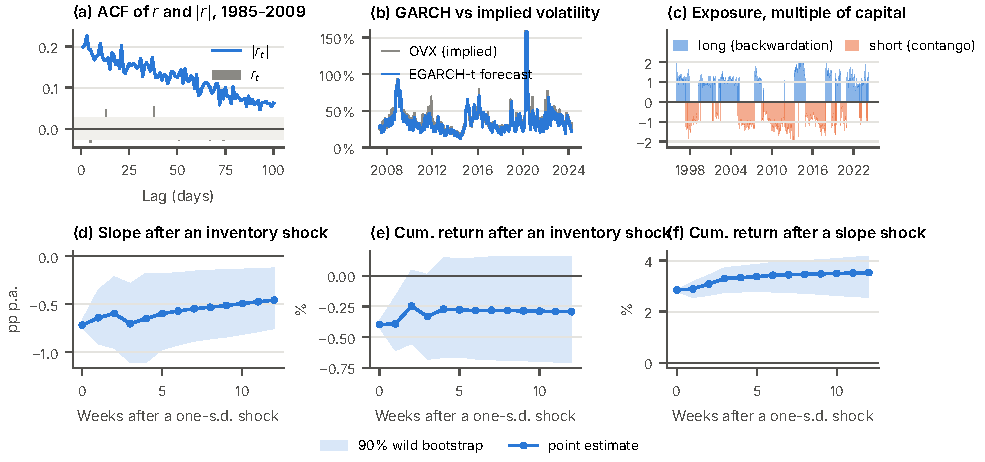
\includegraphics[width=\linewidth]{figures/fig_evidence.pdf}
\caption{(a) Autocorrelations, band $\pm1.96/\sqrt{n}$. (b) EGARCH-$t$ walk-forward forecast against OVX, weekly. (c) Weekly strategy exposure. (d)--(f) Cholesky impulse responses of the VAR(\NVarLags), 1987--2009, with 90\% wild-bootstrap bands (999 draws).}\label{fig:evidence}
\end{figure}

\textbf{Predictability.} H2 holds only in a weak form (Table~\ref{tab:var}). No block of lags is significant in the return equation (joint $p$ \NGrangerAllP). The slope coefficients sum to \NPassSum, which rejects neither zero ($p$ \NPassZeroP) nor full pass-through of the roll yield, $1/52$ per week ($p$ \NPassFullP): weekly returns have a volatility of \NWeeklyVolIs\% against an average absolute roll yield of \NCarryWeekIs\% per week, so the test has little power. The sign of the slope separates the regimes much more clearly, with next-week returns of \NBackAnn\% p.a.\ ($t=\NBackT$) in backwardation and \NContAnn\% p.a.\ ($t=\NContT$) in contango. Walk-forward VAR forecasts lose to the prevailing mean: the out-of-sample $R^2$ \citep{campbell2008} is \NOosRtwoVal{} on validation and \NOosRtwoOos{} on 2010--2024 (Clark--West $p$ \NCwPOos; \citealp{clark2007}), and the hit rate is no better than chance \citep{pesaran1992}. The point forecasts are dominated by the intercept and short-run noise. We therefore trade the regime the VAR identifies, not its point forecast, and keep the VAR forecast as a competing signal.

\begin{table}[t]
\centering\footnotesize
\caption{Return predictability in the weekly VAR(\NVarLags)}\label{tab:var}
\begin{tabular}{@{}lrr@{}}
\toprule
VAR(4) evidence & In-sample & Out-of-sample \\
\midrule
Granger: inventory $\to r$ (HC3 Wald, $p$) & 0.706 &  \\
Granger: slope $\to r$ & 0.635 &  \\
Granger: all lags $\to r$ & 0.374 &  \\
Slope pass-through $\sum_i b_i$ (s.e.) & 0.0078 (0.0111) &  \\
\quad $H_0$: 0 / $H_0$: 1/52 (full carry), $p$ & 0.482 / 0.305 &  \\
Next-week return, backwardation (\% p.a., $t$) & 26.7 (3.1) &  \\
Next-week return, contango (\% p.a., $t$) & \textminus 14.1 (\textminus 1.2) &  \\
\midrule
Out-of-sample $R^2$ vs prevailing mean & \textminus 2.0\% & \textminus 2.6\% \\
Clark--West $p$ (one-sided) & 0.636 & 0.819 \\
Directional hit rate; Pesaran--Timmermann $p$ & 50.7\%; 0.719 & 49.9\%; 0.603 \\
\bottomrule
\end{tabular}

\tabnote{In-sample rows: VAR on 1987--2009, Wald tests with HC3 covariance, regime means with Newey--West $t$ (4 lags). Forecast rows: one-step walk-forward forecasts on validation 1996--2009 (left) and 2010--2024 (right) against the expanding historical mean.}
\end{table}

\section{Strategy selection and validation}
Six candidates take their direction from being always long, from the sign of the VAR forecast or from the sign of the slope, each at 1$\times$ and with the GARCH volatility target (Table~\ref{tab:perf}, top). On 1996--2009 the two carry variants led with Sharpe ratios of \NValSharpeCarry{} and \NValSharpeMain{} and were positive in both seven-year halves; the VAR signal reached \NValSharpeVar{} and \NValSharpeVarVol. The carry variants differ by far less than one standard error, and we chose the volatility-targeted one because the VaR limits in Section~\ref{sec:risk} need a fixed ex-ante risk budget. Correcting for selection over all \NNTrials{} configurations evaluated on validation, the expected best Sharpe ratio of that many unskilled trials is \NDsrHurdle, and the deflated Sharpe ratio \citep{bailey2014}, the probability of beating it, is \NDsr: suggestive, not conclusive \citep{harvey2016}.

\section{Out-of-sample results}
\begin{table}[t]
\centering\footnotesize
\caption{Performance net of costs}\label{tab:perf}
\begin{tabular}{@{}lrrrrrrrr@{}}
\toprule
Strategy & Sharpe & Vol & CAGR & MaxDD & $\alpha$ p.a. & $t(\alpha)$ & $\beta$ & Turnover \\
\midrule
\multicolumn{9}{@{}l}{\textit{Validation 1996--2009}} \\
Long WTI, 1x (benchmark) & 0.50 & 38\% & 14.7\% & \textminus 78\% &  &  &  & 24$\times$ \\
Long WTI, vol-targeted & 0.55 & 36\% & 16.2\% & \textminus 66\% & 2.6\% & 0.8 & 0.90 & 29$\times$ \\
VAR signal, 1x & 0.14 & 38\% & 1.6\% & \textminus 60\% & 2.3\% & 0.2 & 0.15 & 61$\times$ \\
VAR signal, vol-targeted & 0.02 & 36\% & \textminus 1.8\% & \textminus 66\% & \textminus 3.2\% & \textminus 0.3 & 0.20 & 65$\times$ \\
Carry signal, 1x & 0.74 & 38\% & 24.0\% & \textminus 52\% & 28.9\% & 2.7 & \textminus 0.04 & 29$\times$ \\
\textbf{Carry signal, vol-targeted} & 0.70 & 36\% & 21.9\% & \textminus 54\% & 23.7\% & 2.3 & 0.08 & 33$\times$ \\
\midrule
\multicolumn{9}{@{}l}{\textit{Out-of-sample 2010--2024}} \\
Long WTI, 1x (benchmark) & 0.03 & 40\% & \textminus 5.6\% & \textminus 94\% &  &  &  & 24$\times$ \\
Long WTI, vol-targeted & \textminus 0.08 & 36\% & \textminus 7.8\% & \textminus 93\% & \textminus 3.9\% & \textminus 0.9 & 0.81 & 33$\times$ \\
VAR signal, 1x & \textminus 0.23 & 40\% & \textminus 14.8\% & \textminus 96\% & \textminus 9.1\% & \textminus 1.0 & 0.11 & 68$\times$ \\
VAR signal, vol-targeted & \textminus 0.34 & 36\% & \textminus 15.9\% & \textminus 97\% & \textminus 12.2\% & \textminus 1.3 & 0.11 & 82$\times$ \\
Carry signal, 1x & 0.24 & 40\% & 2.7\% & \textminus 73\% & 10.0\% & 1.1 & \textminus 0.46 & 29$\times$ \\
\textbf{Carry signal, vol-targeted} & 0.42 & 36\% & 10.1\% & \textminus 54\% & 15.3\% & 1.7 & \textminus 0.24 & 38$\times$ \\
\bottomrule
\end{tabular}

\tabnote{Sharpe ratio and volatility of daily excess returns over T-bills; CAGR and maximum drawdown of total returns (collateral in T-bills). $\alpha$, $\beta$: regression on benchmark excess returns, Newey--West $t$ (5 lags). Turnover: notional traded per year in multiples of capital, rolls included. Bold: selected on validation.}
\end{table}

From January 2010 to April 2024 the strategy earned a Sharpe ratio of \NOosSharpeMain{} (standard error \NOosSharpeSe; \citealp{opdyke2007}) and \NOosCagrMain{} a year, while the benchmark lost \NOosCagrBench{} a year. Its maximum drawdown was \NOosMddMain, against \NOosMddBench{} (Table~\ref{tab:perf}, Figure~\ref{fig:perf}), with a beta of \NOosBetaMain{} and an annual alpha of \NOosAlphaMain{} ($t=\NOosAlphaT$). The Sharpe ratio was positive in each subperiod: \NSubOne{} (2010--14), \NSubTwo{} (2015--19), \NSubThree{} (2020--24). A stationary bootstrap \citep{politis1994} with 21-day blocks gives a 90\% interval of [\NBootLo, \NBootHi] and $P(\mathrm{SR}\leq 0)=\NBootP$. The gain over the benchmark, \NBootDiff, is not significant (interval [\NBootDiffLo, \NBootDiffHi]), nor is the Sharpe ratio after a Holm correction \citep{holm1979} over the five candidates ($p=\NHolmMain$).

Volatility targeting raised the Sharpe ratio of carry from \NOosSharpeCarry{} to \NOosSharpeMain{} but lowered that of the long position from \NOosSharpeBench{} to \NOosSharpeLongVol: on its own, timing volatility added no return here; it controls risk. The VAR-forecast signal lost money (\NOosSharpeVarVol), in line with its negative out-of-sample $R^2$. The carry return came mostly from contango crashes (Table~\ref{tab:stress}).

\begin{figure}[t]
\centering
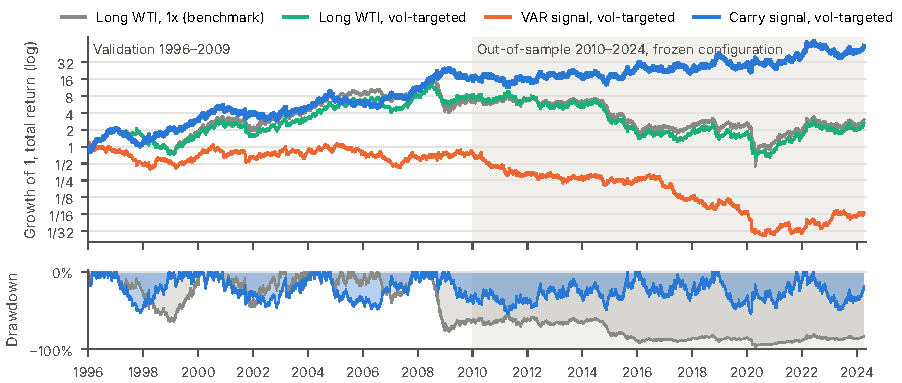
\includegraphics[width=\linewidth]{figures/fig_performance.pdf}
\caption{Growth of one unit of capital (total return, log scale) and drawdowns. Shaded: out-of-sample period, configuration frozen beforehand.}\label{fig:perf}
\end{figure}

\textbf{Robustness.} Changing one setting at a time (Figure~\ref{fig:robust}), the out-of-sample Sharpe ratio ranges from \NRobMin{} to \NRobMax{} across \NRobN{} variants. Five ticks of slippage leave \NRobFiveTicks; a slope from C2/C3 gives \NRobTwoThree. Trading the signal less often hurt: monthly rebalancing \NRobMonthly, a $\pm5\%$ neutral zone \NRobBand. A long/flat version reaches \NRobLongFlat{} with a \NRobLongFlatDd{} drawdown. Every variant scores lower out of sample than on validation, the shrinkage to expect after selection.

\begin{figure}[t]
\centering
\begin{minipage}[t]{0.5\linewidth}\vspace{0pt}
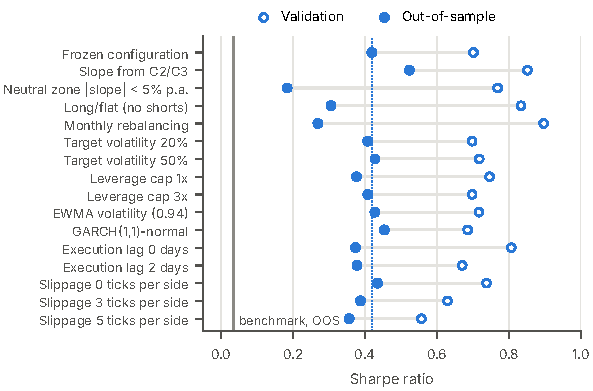
\includegraphics[width=\linewidth]{figures/fig_robustness.pdf}
\captionof{figure}{Robustness: one setting changed at a time. Hollow: validation 1996--2009; filled: 2010--2024. Dotted: frozen configuration; grey: benchmark (both out-of-sample). Full table in Appendix~D.}\label{fig:robust}
\end{minipage}\hfill
\begin{minipage}[t]{0.465\linewidth}\vspace{0pt}
\captionof{table}{Excess returns in oil-market stress episodes}\label{tab:stress}
\centering\footnotesize
\resizebox{\linewidth}{!}{\begin{tabular}{@{}lrrrr@{}}
\toprule
Episode & Bench. & Long v.t. & Carry v.t. & Carry DD \\
\midrule
Asian crisis 1997--98 & \textminus 59\% & \textminus 61\% & 80\% & \textminus 23\% \\
GFC, 2008 H2 & \textminus 69\% & \textminus 48\% & 41\% & \textminus 26\% \\
OPEC price war 2014--16 & \textminus 74\% & \textminus 76\% & 45\% & \textminus 42\% \\
COVID, Jan--Apr 2020 & \textminus 78\% & \textminus 62\% & 20\% & \textminus 34\% \\
Russia--Ukraine 2022 & 23\% & 29\% & 29\% & \textminus 17\% \\
\bottomrule
\end{tabular}
}
\tabnote{Cumulative excess return over each window and the strategy's maximum drawdown within it; v.t.\ = volatility-targeted. The first two episodes fall in the validation period.}
\end{minipage}
\end{figure}

\section{Risk}\label{sec:risk}
One-day EGARCH-$t$ VaR is well calibrated for the strategy: at 1\% the out-of-sample breach rate is \NVarHitMain{} (Kupiec $p$ \NVarKupMain; \citealp{kupiec1995,christoffersen1998}). For the long benchmark it is \NVarHitBench{} (\NVarHitsBench{} breaches in \NVarDaysBench{} days, $p$ \NVarKupBench), spread over the whole period: oil's left tail is heavier than its right (skewness \NSkewOos{} since 2010), which a symmetric $t$ misses for a long position, while the strategy is short about half the time. The historical 99\% expected shortfall is \NOosEsMain{} per day, against \NOosEsBench{} for the benchmark. The main risks are a rally while the curve is in contango, as in 2009 and 2016; gaps between weekly rebalancing dates; and leverage, since the 2$\times$ cap binds when forecast volatility is below 17.5\%, where a 10\% overnight move costs 20\%.

\section{Implementation}
WTI futures are the most liquid crude oil contract, with 983{,}000 contracts traded per day on average in 2024 across all maturities \citep{cme2025}. At 2$\times$ leverage, 100 million USD of capital is about 2{,}700 contracts at 75 USD, roughly 0.3\% of that volume, and can be executed with trade-at-settlement orders at the price the backtest assumes. Turnover is \NOosTurnMain$\times$ capital per year, mostly rolls, and costs take \NOosCostMain{} p.a.\ under our assumptions. A live version needs a licensed price feed, since the EIA no longer publishes settlements.

\section{Limitations and next steps}
The strategy trades one market on one signal and earned most of its excess return in a few contango crashes; without such episodes it would likely have done worse. Costs ignore market impact and assume settlement prices are attainable; historical EIA release times are approximated by a fixed lag; inventory surprises are measured against a seasonal norm, not analyst expectations; the sample ends in April 2024. Next steps are a vendor price series to 2026, carry across several commodities, a combination with time-series momentum, skewed-$t$ VaR for long positions and regime-switching volatility.

{\small
\setlength{\bibsep}{1pt plus 0.3pt}
\bibliography{references}
}

\clearpage
\appendix
\section*{Appendix}
\addcontentsline{toc}{section}{Appendix}
\renewcommand{\thetable}{A\arabic{table}}
\renewcommand{\thefigure}{A\arabic{figure}}
\setcounter{table}{0}
\setcounter{figure}{0}

\subsection*{A\quad Formulas}
\begin{small}
\begin{description}[leftmargin=0pt,itemsep=1pt,font=\normalfont\bfseries]
\item[Rolled return.] $R_t = P^{(2)}_{t}/P^{(2)}_{t-1}-1$ on regular days, $R_t=P^{(1)}_{t}/P^{(2)}_{t-1}-1$ on the first day after an expiry; $P^{(k)}$ is the settlement of the $k$-th contract.
\item[Slope.] $s_t = \tfrac{12}{2}\,\ln\!\big(P^{(2)}_t/P^{(4)}_t\big)$, in \% p.a.
\item[Inventory input.] $\text{inv}_t = 100\,\Delta\ln S_t - \tfrac{1}{5}\sum_{j=1}^{5}100\,\Delta\ln S_{w(t),\,y(t)-j}$, with $w$ the ISO week and $y$ the year of $t$.
\item[EGARCH(1,1)-$t$.] $r_t=\mu+\sigma_t z_t$, $z_t\sim t_\nu$ with unit variance, $\ln\sigma_t^2=\omega+\alpha(|z_{t-1}|-\mathrm{E}|z_{t-1}|)+\gamma z_{t-1}+\beta\ln\sigma^2_{t-1}$.
\item[VAR($p$).] $y_t=c+\sum_{i=1}^{p}A_i y_{t-i}+u_t$, $\mathrm{E}[u_tu_t']=\Sigma=PP'$ with $P$ lower triangular; orthogonalised responses $\Theta_h=\Psi_hP$, generalised responses $\Psi_h\Sigma e_j/\sqrt{\sigma_{jj}}$, where $\Psi_h$ are the moving-average matrices.
\item[Exposure and returns.] $w_t=\operatorname{sign}(s_t)\min(\sigma^*/\hat\sigma_{t+1|t},2)$; daily total return $r^{f}_t+w_{t-1}R_t-c_t$ with costs $c_t=\big(|w_t-w_{t-1}|+2|w_{t-1}|\mathbb{1}_{\text{roll},t}\big)(0.01k+0.0025)/P^{(2)}_t$ for $k$ ticks of slippage.
\item[Sharpe inference.] $\widehat{\mathrm{SE}}(\widehat{\mathrm{SR}})=\sqrt{(1-\hat\gamma_3\widehat{\mathrm{SR}}+\tfrac{\hat\gamma_4-1}{4}\widehat{\mathrm{SR}}^2)/(n-1)}$ \citep{opdyke2007}; $\mathrm{PSR}(\mathrm{SR}^*)=\Phi\big((\widehat{\mathrm{SR}}-\mathrm{SR}^*)/\widehat{\mathrm{SE}}\big)$ \citep{bailey2012}; the deflated Sharpe ratio uses $\mathrm{SR}^*=\sqrt{V[\widehat{\mathrm{SR}}_n]}\big((1-\gamma)\Phi^{-1}(1-\tfrac1N)+\gamma\Phi^{-1}(1-\tfrac{1}{Ne})\big)$ for $N$ trials, $\gamma$ the Euler--Mascheroni constant \citep{bailey2014}.
\item[Forecast and risk tests.] QLIKE loss $\ln h_t+r_t^2/h_t$; Clark--West statistic $f_t=(a_t-b_t)^2-[(a_t-m_t)^2-(b_t-m_t)^2]$ for actual $a$, benchmark $b$ and model $m$; Kupiec $LR_{uc}=-2\ln[(1-\alpha)^{n-x}\alpha^x/((1-\hat\pi)^{n-x}\hat\pi^x)]\sim\chi^2_1$ for $x$ breaches in $n$ days.
\end{description}
\end{small}

\subsection*{B\quad Parameters}
\begin{table}[H]
\centering\small
\caption{Frozen configuration (\texttt{config/strategy.yaml})}
\begin{tabular}{@{}p{0.2\textwidth}p{0.76\textwidth}@{}}
\toprule
Item & Setting \\
\midrule
Instrument & NYMEX WTI futures (CL), 2nd nearby, rolled on front-month expiry \\
Signal & sign of annualised log slope ln(C2/C4), +1 backwardation, $-$1 contango \\
Sizing & target volatility 35\%, EGARCH(1,1)-$t$ 1-day forecast, cap 2$\times$ capital \\
Rebalancing & weekly, last trading day of the week; executed at next settlement \\
Costs & 1 tick (0.01 USD/bbl) slippage + 0.0025 USD/bbl fees per side; rolls charged both legs \\
Volatility model & EGARCH-t, expanding window, refit every 21 trading days \\
VAR & VAR(4) in (inventory, slope, return), expanding window, refit weekly \\
Inventory input & weekly log change minus 5-year same-week mean; usable 6 days after week end \\
Samples & design 1985--2009 (validation 1996--2009); out-of-sample 2010-01--2024-04 \\
\bottomrule
\end{tabular}

\end{table}

\subsection*{C\quad Data}
\begin{table}[H]
\centering\small
\caption{Raw data files, as downloaded on 15 November 2026 (\texttt{data/raw/MANIFEST.json})}
\begin{tabular}{@{}p{0.27\textwidth}p{0.5\textwidth}l@{}}
\toprule
File & Content & SHA-256 (first 12) \\
\midrule
\texttt{eia\_RCLC1d.xls} & NYMEX WTI futures, contract 1, daily settle (USD/bbl) & \texttt{021180c292ab} \\
\texttt{eia\_RCLC2d.xls} & NYMEX WTI futures, contract 2, daily settle (USD/bbl) & \texttt{dc8fd7856e08} \\
\texttt{eia\_RCLC3d.xls} & NYMEX WTI futures, contract 3, daily settle (USD/bbl) & \texttt{249839d65d6d} \\
\texttt{eia\_RCLC4d.xls} & NYMEX WTI futures, contract 4, daily settle (USD/bbl) & \texttt{c57062b38077} \\
\texttt{eia\_RWTCd.xls} & WTI spot price, Cushing, daily (USD/bbl) & \texttt{97903eda6ea2} \\
\texttt{eia\_WCESTUS1w.xls} & US crude oil ending stocks excl. SPR, weekly (kbbl) & \texttt{1841caa0cc6f} \\
\texttt{eia\_cushing\_stocks\_w.xls} & Cushing crude oil ending stocks excl. SPR, weekly (kbbl) & \texttt{7dbe4f72766d} \\
\texttt{fred\_DTB3.csv} & 3-month T-bill, secondary market, daily (\% p.a.) & \texttt{e348dc53e133} \\
\texttt{fred\_OVXCLS.csv} & CBOE crude oil ETF volatility index, daily & \texttt{0ddd2b2d5801} \\
\bottomrule
\end{tabular}

\tabnote{Sources: \citet{eiafutures}, \citet{eiastocks}, \citet{fred}. Cushing stocks and the spot price were downloaded for reference and are not used in the strategy.}
\end{table}

\subsection*{D\quad Additional results}
\begin{table}[H]
\centering\small
\begin{minipage}[t]{0.47\linewidth}\centering
\caption{GARCH specifications, 1985--2009}\label{tab:volspecs}
\resizebox{\linewidth}{!}{\begin{tabular}{@{}lrrrr@{}}
\toprule
Model & BIC & Persistence & $\gamma$ ($t$) & $\nu$ \\
\midrule
GARCH-N & 23\,617 & 0.998 &  &  \\
GARCH-t & 23\,367 & 0.998 &  & 6.7 \\
GJR-t & 23\,369 & 0.997 & 0.026 (2.4) & 6.7 \\
EGARCH-t & 23\,330 & 0.991 & \textminus 0.027 (\textminus 3.9) & 6.8 \\
GJR-skewt & 23\,368 & 0.997 & 0.027 (2.5) & 6.8 \\
\bottomrule
\end{tabular}
}
\tabnote{Persistence: $\alpha+\beta+\gamma/2$ (GARCH, GJR) or $\beta$ (EGARCH). $\gamma$: asymmetry coefficient, robust $t$ in brackets.}
\end{minipage}\hfill
\begin{minipage}[t]{0.5\linewidth}\centering
\caption{One-day variance forecasts}\label{tab:voleval}
\resizebox{\linewidth}{!}{\begin{tabular}{@{}lrrrr@{}}
\toprule
1-day forecast & QLIKE & DM $t$ [$p$] & QLIKE & DM $t$ [$p$] \\
\midrule
EGARCH-t & 2.659 & -- & 2.403 & -- \\
GARCH-N & 2.670 & \textminus 3.0 [0.002] & 2.411 & \textminus 1.0 [0.316] \\
EWMA & 2.668 & \textminus 1.6 [0.109] & 2.438 & \textminus 3.6 [$<$0.001] \\
Rolling 63d & 2.672 & \textminus 1.2 [0.221] & 2.533 & \textminus 3.8 [$<$0.001] \\
\bottomrule
\end{tabular}
}
\tabnote{Left: validation 1996--2009; right: 2010--2024. Diebold--Mariano test of EGARCH-$t$ against each model on QLIKE loss (Newey--West, 5 lags); negative $t$ favours EGARCH-$t$.}
\end{minipage}
\end{table}

\begin{table}[H]
\centering\small
\caption{One-at-a-time robustness}\label{tab:robust}
\begin{tabular}{@{}llrrrr@{}}
\toprule
Dimension & Variant & Sharpe val. & Sharpe OOS & MaxDD OOS & Turnover OOS \\
\midrule
Baseline & Frozen configuration & 0.70 & 0.42 & \textminus 54\% & 38 \\
\midrule
Signal & Slope from C2/C3 & 0.85 & 0.52 & \textminus 45\% & 38 \\
 & Neutral zone $|s| <$ 5\% p.a. & 0.77 & 0.18 & \textminus 62\% & 30 \\
 & Long/flat (no shorts) & 0.83 & 0.31 & \textminus 43\% & 17 \\
\midrule
Rebalancing & Monthly & 0.90 & 0.27 & \textminus 62\% & 34 \\
\midrule
Target volatility & 20\% & 0.70 & 0.41 & \textminus 34\% & 22 \\
 & 50\% & 0.72 & 0.43 & \textminus 68\% & 50 \\
\midrule
Leverage cap & 1x & 0.75 & 0.38 & \textminus 48\% & 28 \\
 & 3x & 0.70 & 0.41 & \textminus 54\% & 39 \\
\midrule
Volatility model & EWMA (0.94) instead of EGARCH-t & 0.72 & 0.43 & \textminus 54\% & 40 \\
 & GARCH(1,1)-normal & 0.69 & 0.45 & \textminus 53\% & 40 \\
\midrule
Execution lag & 0 days & 0.81 & 0.37 & \textminus 52\% & 38 \\
 & 2 days & 0.67 & 0.38 & \textminus 50\% & 38 \\
\midrule
Slippage & 0 ticks per side & 0.74 & 0.44 & \textminus 54\% & 38 \\
 & 3 ticks per side & 0.63 & 0.39 & \textminus 55\% & 38 \\
 & 5 ticks per side & 0.56 & 0.36 & \textminus 56\% & 38 \\
\midrule
VAR signal & Frozen VAR(4) & 0.02 & \textminus 0.34 & \textminus 97\% & 82 \\
 & VAR(1) & 0.37 & 0.05 & \textminus 88\% & 64 \\
 & VAR(8) & 0.20 & \textminus 0.37 & \textminus 96\% & 76 \\
 & Rolling 10-year window & \textminus 0.05 & \textminus 0.15 & \textminus 82\% & 79 \\
 & Without inv & 0.09 & \textminus 0.27 & \textminus 97\% & 80 \\
 & Without slope & 0.21 & \textminus 0.30 & \textminus 98\% & 76 \\
\bottomrule
\end{tabular}

\tabnote{Rows above the VAR block vary the selected carry strategy; the VAR block varies the specification behind the competing VAR-signal strategy. Turnover in multiples of capital per year.}
\end{table}

\begin{table}[H]
\centering\small
\caption{Backtest of one-day EGARCH-$t$ Value-at-Risk, 2010--2024}
\begin{tabular}{@{}llrrrr@{}}
\toprule
Position & $\alpha$ & Hits / days & Hit rate & Kupiec $p$ & Christoffersen $p$ \\
\midrule
Long WTI, 1x & 1\% & 55 / 3574 & 1.54\% & 0.003 & 0.063 \\
Long WTI, 1x & 5\% & 215 / 3574 & 6.02\% & 0.007 & 0.051 \\
Carry signal, vol-targeted & 1\% & 26 / 3560 & 0.73\% & 0.089 & 0.536 \\
Carry signal, vol-targeted & 5\% & 154 / 3560 & 4.33\% & 0.059 & 0.892 \\
\bottomrule
\end{tabular}

\end{table}

\begin{figure}[H]
\centering
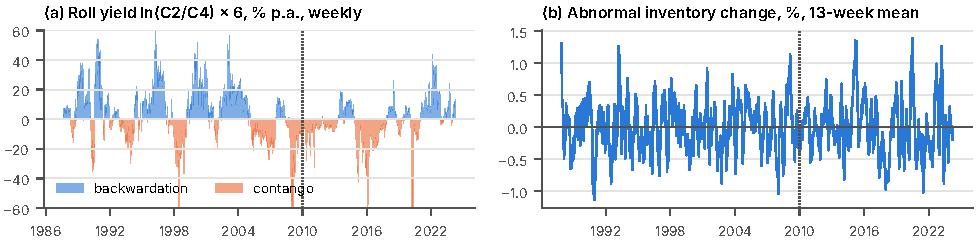
\includegraphics[width=\linewidth]{figures/fig_inputs.pdf}
\caption{Signal inputs. Dotted line: start of the out-of-sample period.}
\end{figure}

\begin{figure}[H]
\centering
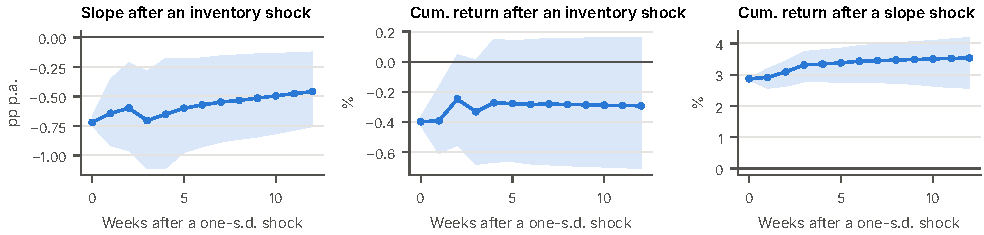
\includegraphics[width=\linewidth]{figures/fig_girf.pdf}
\caption{Generalised impulse responses \citep{pesaran1998}, same VAR and bootstrap as Figure~\ref{fig:evidence}.}
\end{figure}

\begin{figure}[H]
\centering
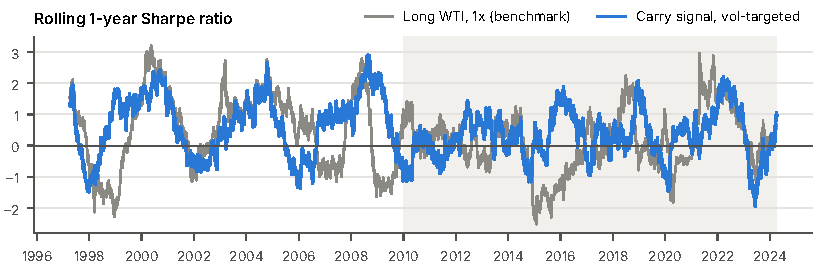
\includegraphics[width=\linewidth]{figures/fig_rolling_sharpe.pdf}
\caption{Rolling one-year Sharpe ratio of the strategy and the benchmark; shaded: out-of-sample period.}
\end{figure}

\subsection*{E\quad Reproducibility}
\begin{small}
All results are produced by the code in the project repository. \texttt{python scripts/download\_data.py} stores the raw files; \texttt{python -m wti.analysis} runs the models and backtests; \texttt{python -m wti.report} writes every table, figure and every number quoted in the text (\texttt{reports/tables/numbers.tex}); \texttt{pytest} runs the tests, including the look-ahead checks.
\end{small}

\end{document}
